\documentclass[12pt,a4paper]{article}

% ─── Page Layout ───────────────────────────────────────────────────────────────
\usepackage[a4paper, margin=0.8in, headheight=14pt]{geometry}

% ─── Fonts (XeLaTeX) ───────────────────────────────────────────────────────────
\usepackage{fontspec}
\usepackage{unicode-math}
\setmainfont{TeX Gyre Pagella}
\setmonofont[Scale=0.88]{TeX Gyre Cursor}
\setmathfont{Latin Modern Math}

% ─── Packages ──────────────────────────────────────────────────────────────────
\usepackage{xcolor}
\usepackage{colortbl}
\usepackage{titlesec}
\usepackage{enumitem}
\usepackage{tabularx}
\usepackage{booktabs}
\usepackage{array}
\usepackage{amsmath}
\usepackage{tikz}
\usetikzlibrary{shapes.geometric, arrows.meta, positioning, calc, fit, decorations.pathreplacing}
\usepackage{tcolorbox}
\tcbuselibrary{skins, breakable}
\usepackage{hyperref}
\usepackage{fancyhdr}
\usepackage{graphicx}
\usepackage{microtype}
\hyphenpenalty=10000
\exhyphenpenalty=10000
\sloppy
\usepackage{caption}
\usepackage{setspace}
\usepackage{multirow}
\usepackage{tocloft}

% ─── Q&A helper ────────────────────────────────────────────────────────────────
\newcommand{\Q}[1]{\textbf{#1}\par\noindent\ignorespaces}

% ─── Colour Palette ────────────────────────────────────────────────────────────
\definecolor{myred}{RGB}{196,30,58}
\definecolor{mydark}{RGB}{30,30,50}
\definecolor{mygreen}{RGB}{14,120,80}
\definecolor{myteal}{RGB}{0,130,140}
\definecolor{myamber}{RGB}{180,100,0}
\definecolor{mypurple}{RGB}{100,30,160}
\definecolor{mygray}{RGB}{246,247,249}
\definecolor{mgframe}{RGB}{180,185,200}
\definecolor{watermark}{RGB}{145,150,170}
\definecolor{hdrred}{RGB}{250,232,235}
\definecolor{hdrgreen}{RGB}{220,244,233}
\definecolor{hdrteal}{RGB}{220,242,244}
\definecolor{hdramber}{RGB}{253,242,215}
\definecolor{hdrpurple}{RGB}{238,228,255}
\definecolor{hdrgray}{RGB}{238,240,245}
\definecolor{rowalt}{RGB}{250,251,253}

% ─── Section Formatting ────────────────────────────────────────────────────────
\titleformat{\section}
  {\large\bfseries\color{myred}}{\thesection.}{0.5em}{}
  [\vspace{1pt}{\color{myred}\rule{\linewidth}{0.8pt}}]
\titleformat{\subsection}
  {\normalsize\bfseries\color{myteal}}{\thesubsection}{0.5em}{}
\titlespacing*{\section}{0pt}{18pt}{7pt}
\titlespacing*{\subsection}{0pt}{11pt}{4pt}

% ─── Paragraph ─────────────────────────────────────────────────────────────────
\setlength{\parindent}{0pt}
\setlength{\parskip}{4pt}

% ─── TOC Styling ───────────────────────────────────────────────────────────────
\renewcommand{\cfttoctitlefont}{\large\bfseries\color{myred}}
\renewcommand{\cftaftertoctitle}{\par\noindent{\color{myred}\rule{\linewidth}{0.8pt}}}
\setlength{\cftbeforetoctitleskip}{0pt}
\setlength{\cftaftertoctitleskip}{6pt}
\renewcommand{\cftsecfont}{\normalsize\bfseries\color{mydark}}
\renewcommand{\cftsecpagefont}{\normalsize\bfseries\color{mydark}}
\renewcommand{\cftsecleader}{\cftdotfill{\cftdotsep}}
\setlength{\cftbeforesecskip}{7pt}
\renewcommand{\cftsubsecfont}{\small\color{mydark}}
\renewcommand{\cftsubsecpagefont}{\small\color{mydark}}
\setlength{\cftbeforesubsecskip}{3pt}
\setlength{\cftsubsecindent}{1.4em}

% ─── Table helpers ─────────────────────────────────────────────────────────────
\renewcommand{\arraystretch}{1.45}
\setlength{\tabcolsep}{6pt}
\arrayrulecolor{mydark}
\newcolumntype{B}[1]{>{\small\bfseries\raggedright\arraybackslash}m{#1}}
\newcolumntype{Y}{>{\small\raggedright\arraybackslash}X}
\renewcommand{\tabularxcolumn}[1]{m{#1}}

% ─── Header / Footer ───────────────────────────────────────────────────────────
\pagestyle{fancy}
\fancyhf{}
\fancyhead[L]{\small\color{myred}\textbf{EC301}\;\color{mydark}--- Electronic Devices}
\fancyhead[R]{\small\color{myteal}\textbf{Module 4 Notes}}
\fancyfoot[C]{\small\color{mydark}\thepage}
\fancyfoot[R]{\small\color{watermark}\textit{\copyright\ Biraj}}
\renewcommand{\headrulewidth}{0.5pt}
\renewcommand{\footrulewidth}{0.3pt}

% ─── Hyperref ──────────────────────────────────────────────────────────────────
\hypersetup{
  colorlinks=true, linkcolor=myteal, urlcolor=myteal,
  pdfauthor={Biraj Sarkar (CGEC)},
  pdftitle={EC301 --- Module 4 Notes: Opto-Electronics and IC Fabrication}
}

% ─── tcolorbox styles ──────────────────────────────────────────────────────────
\tcbset{
  tikzbox/.style={
    colback=mygray, colframe=mgframe, boxrule=0.6pt, arc=4pt,
    left=8pt, right=8pt, top=6pt, bottom=6pt,
    colbacktitle=mgframe, coltitle=mydark,
    fonttitle=\small\bfseries
  },
  defbox/.style={
    colback=hdrgreen, colframe=mygreen, boxrule=0.8pt, arc=4pt,
    left=9pt, right=9pt, top=6pt, bottom=6pt,
    colbacktitle=mygreen, coltitle=white,
    fonttitle=\small\bfseries
  },
  formulabox/.style={
    colback=hdrteal, colframe=myteal, boxrule=0.8pt, arc=4pt,
    left=9pt, right=9pt, top=7pt, bottom=7pt,
    colbacktitle=myteal, coltitle=white,
    fonttitle=\small\bfseries
  },
  examplebox/.style={
    colback=hdramber, colframe=myamber, boxrule=0.8pt, arc=4pt,
    left=9pt, right=9pt, top=6pt, bottom=6pt,
    colbacktitle=myamber, coltitle=white,
    fonttitle=\small\bfseries
  },
  masonbox/.style={
    colback=hdrpurple, colframe=mypurple, boxrule=0.8pt, arc=4pt,
    left=9pt, right=9pt, top=6pt, bottom=6pt,
    colbacktitle=mypurple, coltitle=white,
    fonttitle=\small\bfseries
  },
  exambox/.style={
    colback=hdrpurple, colframe=mypurple, boxrule=1pt, arc=5pt,
    left=10pt, right=10pt, top=8pt, bottom=8pt,
    colbacktitle=mypurple, coltitle=white,
    fonttitle=\bfseries,
    breakable, title after break={\textbf{Frequently Asked / Viva Questions (contd.)}}}
}
\tcbset{breakable}

% ─── TikZ styles ───────────────────────────────────────────────────────────────
\tikzset{
  block/.style={rectangle, draw=myteal, fill=hdrteal,
    text width=2.4cm, align=center, minimum height=0.95cm,
    font=\small, rounded corners=3pt, line width=0.7pt},
  redblock/.style={rectangle, draw=myred, fill=hdrred,
    text width=2.4cm, align=center, minimum height=0.95cm,
    font=\small, rounded corners=3pt, line width=0.7pt},
  greenblock/.style={rectangle, draw=mygreen, fill=hdrgreen,
    text width=2.4cm, align=center, minimum height=0.95cm,
    font=\small, rounded corners=3pt, line width=0.7pt},
  amberblock/.style={rectangle, draw=myamber, fill=hdramber,
    text width=2.4cm, align=center, minimum height=0.95cm,
    font=\small, rounded corners=3pt, line width=0.7pt},
  purpblock/.style={rectangle, draw=mypurple, fill=hdrpurple,
    text width=2.4cm, align=center, minimum height=0.95cm,
    font=\small, rounded corners=3pt, line width=0.7pt},
  arrow/.style={-Stealth, thick, color=mydark},
  redarrow/.style={-Stealth, thick, color=myred},
  line/.style={thick, color=mydark}
}

% ═══════════════════════════════════════════════════════════════════════════════
\begin{document}
% ═══════════════════════════════════════════════════════════════════════════════

\begin{center}
  {\LARGE\bfseries\color{myred} EC301 --- Electronic Devices}\\[5pt]
  {\normalsize\color{mydark} Semester III \quad$\bullet$\quad 3L:0T:0P \quad$\bullet$\quad 3 Credits}\\[3pt]
  {\normalsize\color{myteal}\textbf{Module 4 Exam Notes: Opto-Electronics \& IC Fabrication Process}}\\[3pt]
  {\small\color{mydark} CGEC \;$|$\; B.Tech ECE (2023--27) \;$|$\; \textit{Biraj Sarkar}}
\end{center}
\vspace{2pt}
\noindent{\color{myred}\rule{\linewidth}{1.5pt}}
\vspace{2pt}

\hypersetup{linkcolor=mydark}
\tableofcontents
\hypersetup{linkcolor=myteal}
\newpage

% ===============================================================================
\section{Optical Absorption in Semiconductors}
% ===============================================================================

Optoelectronic devices operate via the conversion of optical energy (photons) into electrical energy (electrons and holes), or vice versa.

\subsection{Fundamental Optical Absorption Process}
When incident photons strike a semiconductor:
\begin{itemize}[leftmargin=*, itemsep=3pt]
  \item If photon energy is less than the bandgap ($h\nu < E_g$), the semiconductor cannot absorb the photon; the material is transparent to that wavelength.
  \item If photon energy equals or exceeds the bandgap ($h\nu \ge E_g$), the photon is absorbed, elevating a valence electron into the conduction band and creating an \textbf{electron-hole pair (EHP)}.
  \item The \textbf{cut-off wavelength} ($\lambda_c$) above which no band-to-band optical absorption can occur is:
  \begin{equation}
    \lambda_c = \frac{hc}{E_g} = \frac{1.24}{E_g\,(\text{eV})}\,\mu\text{m}
  \end{equation}
  For Silicon ($E_g = 1.12\,\text{eV}$), $\lambda_c \approx 1.11\,\mu\text{m}$ (near infrared). For GaAs ($E_g = 1.42\,\text{eV}$), $\lambda_c \approx 0.87\,\mu\text{m}$.
\end{itemize}

\subsection{Absorption Coefficient and Beer-Lambert's Law}
The attenuation of optical intensity $I(x)$ as light propagates through a distance $x$ within a semiconductor is described by the \textbf{Beer-Lambert Law}:

\begin{tcolorbox}[formulabox, title={\textbf{Beer-Lambert Absorption Law}}]
\begin{equation}
  I(x) = I_0 \exp(-\alpha x)
\end{equation}
where $I_0$ is the incident light intensity (after surface reflection), and $\alpha$ is the \textbf{absorption coefficient} ($\text{cm}^{-1}$). The characteristic \textbf{optical penetration depth} is $\delta = 1/\alpha$. Direct bandgap semiconductors exhibit very steep absorption edges ($\alpha \sim 10^4\text{--}10^5\,\text{cm}^{-1}$, $\delta \sim 0.1\text{--}1\,\mu\text{m}$), whereas indirect bandgap semiconductors require phonon assistance ($\alpha \sim 10^2\text{--}10^3\,\text{cm}^{-1}$, $\delta \sim 10\text{--}100\,\mu\text{m}$).
\end{tcolorbox}

% ===============================================================================
\section{Photovoltaic Effects and Solar Cells}
% ===============================================================================

A \textbf{solar cell} is an un-biased, large-area p-n junction that converts optical solar radiation directly into electrical power via the \textbf{photovoltaic effect}.

\subsection{Physical Working Principle}
\begin{enumerate}[label=\arabic*., leftmargin=*]
  \item Photons with $h\nu \ge E_g$ penetrate the thin top layer and generate EHPs within and adjacent to the space charge depletion layer.
  \item The high built-in electric field $\vec{\mathcal{E}}$ in the depletion region sweeps photogenerated electrons to the n-side and photogenerated holes to the p-side before they can recombine.
  \item This accumulation of charges establishes a forward photovoltage across the terminals, driving an external load current.
\end{enumerate}

\subsection{Equivalent Circuit and Solar Cell I-V Characteristics}
An ideal solar cell is modeled as an ideal light-generated constant current source $I_L$ in parallel with a forward-biased diode:

\begin{tcolorbox}[formulabox, title={\textbf{Solar Cell Current-Voltage Equation}}]
\begin{equation}
  I = I_L - I_D = I_L - I_0 \left[ \exp\left(\frac{q V}{\eta k T}\right) - 1 \right]
\end{equation}
where $I_L$ is the photogenerated current ($I_L \propto \text{incident optical power}$).
\end{tcolorbox}

\begin{tcolorbox}[tikzbox, title={Solar Cell Equivalent Circuit and Fourth-Quadrant I-V Curve}]
\centering
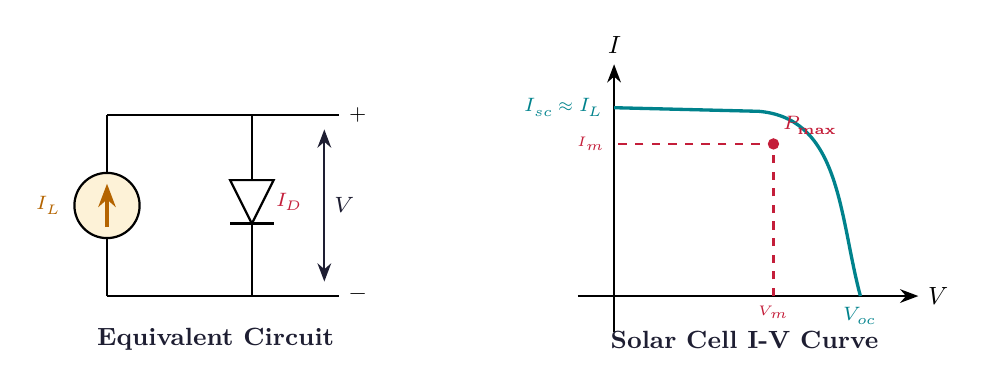
\begin{tikzpicture}[scale=0.92]
  % Equivalent Circuit (Left)
  \begin{scope}[xshift=-4.5cm]
    % Current source IL
    \draw[thick] (0, 0) -- (0, 0.8);
    \draw[thick, fill=hdramber] (0, 1.25) circle (0.45);
    \draw[-Stealth, very thick, color=myamber] (0, 0.95) -- (0, 1.55);
    \node[left, font=\scriptsize\bfseries\color{myamber}] at (-0.5, 1.25) {$I_L$};
    \draw[thick] (0, 1.7) -- (0, 2.5);

    % Diode
    \draw[thick] (0, 2.5) -- (2.0, 2.5) -- (2.0, 1.6);
    \draw[thick] (1.7, 1.6) -- (2.3, 1.6) -- (2.0, 1.0) -- cycle;
    \draw[thick] (1.7, 1.0) -- (2.3, 1.0);
    \draw[thick] (2.0, 1.0) -- (2.0, 0) -- (0, 0);
    \node[right, font=\scriptsize\bfseries\color{myred}] at (2.2, 1.3) {$I_D$};

    % Terminals
    \draw[thick] (2.0, 2.5) -- (3.2, 2.5) node[right, font=\footnotesize\bfseries] {$+$};
    \draw[thick] (2.0, 0) -- (3.2, 0) node[right, font=\footnotesize\bfseries] {$-$};
    \draw[Stealth-Stealth, thick, color=mydark] (3.0, 2.3) -- (3.0, 0.2) node[midway, right, font=\footnotesize\bfseries] {$V$};
    \node[font=\small\bfseries\color{mydark}] at (1.5, -0.6) {Equivalent Circuit};
  \end{scope}

  % I-V Characteristics (Right)
  \begin{scope}[xshift=2.5cm]
    \draw[-Stealth, thick] (-0.5, 0) -- (4.2, 0) node[right, font=\small] {$V$};
    \draw[-Stealth, thick] (0, -0.5) -- (0, 3.2) node[above, font=\small] {$I$};

    % I-V curve
    \draw[very thick, color=myteal] (0, 2.6) node[left, font=\scriptsize\bfseries] {$I_{sc} \approx I_L$} -- (2.0, 2.55) to[out=-5, in=105] (3.4, 0) node[below, font=\scriptsize\bfseries] {$V_{oc}$};

    % Maximum Power Rectangle
    \draw[dashed, thick, color=myred] (2.2, 0) -- (2.2, 2.1) -- (0, 2.1);
    \node[below, font=\tiny\bfseries\color{myred}] at (2.2, 0) {$V_m$};
    \node[left, font=\tiny\bfseries\color{myred}] at (0, 2.1) {$I_m$};
    \filldraw[color=myred] (2.2, 2.1) circle (2pt) node[above right, font=\scriptsize\bfseries] {$P_{\text{max}}$};
    \node[font=\small\bfseries\color{mydark}] at (1.8, -0.6) {Solar Cell I-V Curve};
  \end{scope}
\end{tikzpicture}
\end{tcolorbox}

\subsection{Key Solar Cell Figures of Merit}
\begin{itemize}[leftmargin=*, itemsep=3.5pt]
  \item \textbf{Short-Circuit Current ($I_{sc}$):} Current flowing when terminals are shorted ($V = 0$):
  \begin{equation}
    I_{sc} = I_L
  \end{equation}
  \item \textbf{Open-Circuit Voltage ($V_{oc}$):} Voltage when terminals are open ($I = 0$):
  \begin{equation}
    0 = I_L - I_0 \left[ \exp\left(\frac{q V_{oc}}{\eta k T}\right) - 1 \right] \implies V_{oc} = \eta V_T \ln\left(\frac{I_L}{I_0} + 1\right)
  \end{equation}
  \item \textbf{Maximum Power Point ($P_{\text{max}}$):} Occurs at the knee of the curve where the product $V \cdot I$ is maximized:
  \begin{equation}
    P_{\text{max}} = V_m I_m
  \end{equation}
  \item \textbf{Fill Factor ($FF$):} The ratio of maximum usable power to the theoretical maximum product $V_{oc} I_{sc}$:
  \begin{equation}
    FF = \frac{V_m I_m}{V_{oc} I_{sc}} \quad (\text{typically } 0.70\text{--}0.85)
  \end{equation}
  \item \textbf{Power Conversion Efficiency ($\eta$):}
  \begin{equation}
    \eta = \frac{P_{\text{max}}}{P_{\text{in}}} = \frac{V_{oc} I_{sc} FF}{P_{\text{in}}}
  \end{equation}
  where $P_{\text{in}}$ is the incident solar optical power ($100\,\text{mW/cm}^2$ under AM1.5 standard illumination).
\end{itemize}

% ===============================================================================
\section{Photodetectors: Photoconductors, Photodiodes, PIN and APD}
% ===============================================================================

\subsection{Photoconductors}
A photoconductor is a slab of semiconductor with ohmic contacts at both ends. Light absorption creates excess electron-hole pairs ($\Delta n = \Delta p = g_L \tau$), increasing the material's bulk conductivity:

\begin{equation}
  \Delta \sigma = q (\mu_n + \mu_p) \Delta n = q (\mu_n + \mu_p) g_L \tau
\end{equation}

The \textbf{photoconductive gain} ($G$) is the number of charge carriers passing through the external circuit per absorbed photon:
\begin{equation}
  G = \frac{\tau}{t_{\text{transit}}} = \frac{\tau \mu_n \mathcal{E}}{L} = \frac{\tau \mu_n V}{L^2}
\end{equation}
Because electron lifetime $\tau$ can be much longer than transit time $t_{\text{transit}}$, an electron can circulate through the device multiple times before recombining, producing $G \gg 1$.

\subsection{P-N Photodiode}
A p-n junction operated under \textbf{reverse bias}:
\begin{itemize}[leftmargin=*, itemsep=3pt]
  \item Reverse bias extends the depletion width and creates a high electric field that sweeps photogenerated carriers out rapidly, generating a drift photocurrent:
  \begin{equation}
    I_{\text{total}} = I_0 \left( e^{-V_R / V_T} - 1 \right) - I_{\text{photo}} \approx - (I_0 + I_{\text{photo}})
  \end{equation}
  \item \textbf{Responsivity ($R$):}
  \begin{equation}
    R = \frac{I_{\text{photo}}}{P_{\text{opt}}} = \frac{\eta_{ext} q}{h\nu} = \frac{\eta_{ext} q \lambda}{hc} \quad (\text{A/W})
  \end{equation}
  where $\eta_{ext}$ is the external quantum efficiency.
\end{itemize}

\subsection{PIN Photodiode}
A PIN photodiode inserts a wide, undoped \textbf{intrinsic ($i$)} semiconductor layer between heavily doped $p^+$ and $n^+$ regions ($p^+\text{--}i\text{--}n^+$).

\begin{itemize}[leftmargin=*, itemsep=3pt]
  \item Even under small reverse bias, the intrinsic layer is completely depleted ($W \approx W_i$).
  \item \textbf{Key Advantages over standard p-n photodiodes}:
    \begin{enumerate}
      \item \textbf{High Quantum Efficiency:} The wide $W_i$ provides a large volume for optical absorption, ensuring that nearly all incident photons are converted into drift carriers rather than slow diffusion carriers.
      \item \textbf{Low Junction Capacitance:} Because $C_j = \frac{\epsilon_s A}{W_i}$ and $W_i$ is large, capacitance is extremely small ($< 1\,\text{pF}$), drastically reducing the $RC$ time constant.
      \item \textbf{High Speed / Bandwidth:} Operating speeds reach $10\text{--}40\,\text{GHz}$, making PIN diodes standard in fiber-optic communications.
    \end{enumerate}
\end{itemize}

\subsection{Avalanche Photodiode (APD)}
The APD is operated under very high reverse bias close to the avalanche breakdown voltage:
\begin{itemize}[leftmargin=*, itemsep=3pt]
  \item Photo-generated electrons entering the high-field multiplication depletion region acquire sufficient kinetic energy to cause \textbf{impact ionization}, knocking valence electrons into the conduction band.
  \item This secondary carrier multiplication yields an internal current gain $M$:
  \begin{equation}
    M = \frac{I_{\text{out}}}{I_{\text{photo}}} \approx \frac{1}{1 - (V_R / V_{BR})^n} \quad (M \sim 10\text{--}1000)
  \end{equation}
  \item APDs provide superior optical sensitivity for detecting ultra-weak light signals, but introduce avalanche excess noise.
\end{itemize}

\subsection{Phototransistor}
A phototransistor is a BJT whose reverse-biased collector-base junction is exposed to light. Photogenerated base current $I_{\text{photo}}$ acts as base drive, which is multiplied by the transistor current gain:
\begin{equation}
  I_C = (\beta + 1) I_{\text{photo}}
\end{equation}
It provides high optical sensitivity without external amplifiers, but has lower switching speed than PIN photodiodes due to base charge storage.

% ===============================================================================
\section{Light Emitting Diodes and Semiconductor Lasers}
% ===============================================================================

\subsection{Light Emitting Diode (LED)}
An LED is a heavily doped, forward-biased \textbf{direct bandgap} p-n junction (e.g., $\text{GaAs}, \text{GaN}, \text{InGaN}$).
\begin{itemize}[leftmargin=*, itemsep=3pt]
  \item Forward bias injects minority electrons into the p-side and minority holes into the n-side.
  \item Carriers undergo \textbf{spontaneous radiative recombination}, releasing energy as photons:
  \begin{equation}
    \lambda \approx \frac{hc}{E_g} = \frac{1.24}{E_g\,(\text{eV})}\,\mu\text{m}
  \end{equation}
  \item Emits \textbf{incoherent}, non-directional light across a spectral bandwidth $\Delta \lambda \approx 20\text{--}50\,\text{nm}$.
\end{itemize}

\subsection{Semiconductor Laser Diode}
A laser diode produces \textbf{coherent, monochromatic, and highly directional} optical radiation.

\begin{enumerate}[label=\arabic*., leftmargin=*]
  \item \textbf{Three Radiation Processes:}
    \begin{itemize}
      \item \textbf{Stimulated Absorption:} An incoming photon ($h\nu \approx E_g$) is absorbed, exciting an electron from VB to CB.
      \item \textbf{Spontaneous Emission:} An electron drops spontaneously to the VB, emitting an incoherent photon of random phase and direction.
      \item \textbf{Stimulated Emission:} An incident photon stimulates an excited electron in the CB to drop to the VB, emitting a second photon having the \textbf{exact same energy, phase, polarization, and direction} as the stimulating photon.
    \end{itemize}

  \item \textbf{Population Inversion (Bernard-Duraffourg Condition):}
  To achieve net optical gain (stimulated emission exceeding stimulated absorption), the upper CB states must be more populated than lower VB states. This requires heavy forward current injection such that the separation of quasi-Fermi levels exceeds the photon energy:
  \begin{equation}
    E_g < h\nu < E_{Fn} - E_{Fp}
  \end{equation}

  \item \textbf{Optical Cavity (Fabry-Perot Resonator):}
  Cleaved, polished semiconductor crystal facets at both ends act as partially reflecting mirrors, creating an optical feedback cavity that sustains oscillation above the \textbf{threshold current} $I_{th}$.
\end{enumerate}

% ===============================================================================
\section{Integrated Circuit Fabrication Technologies}
% ===============================================================================

Modern Silicon integrated circuits are manufactured on high-purity single-crystal Silicon wafers using sequential planar processing steps:

\subsection{Overview of Unit Fabrication Steps}
\par\vspace{6pt}\noindent
\begingroup
\setlength{\tabcolsep}{5pt}
\setlength{\extrarowheight}{3pt}
\renewcommand{\arraystretch}{1.35}
\begin{tabularx}{\linewidth}{|B{3.2cm}|Y|Y|}
\hline
\multicolumn{1}{|c|}{\textbf{Process Step}} & \multicolumn{1}{c|}{\textbf{Chemical / Physical Principle}} & \multicolumn{1}{c|}{\textbf{Role in IC Manufacturing}} \\
\hline
Thermal Oxidation & $\text{Si} + \text{O}_2 \to \text{SiO}_2$ (Dry) \newline $\text{Si} + 2\text{H}_2\text{O} \to \text{SiO}_2 + 2\text{H}_2$ (Wet) & Creates gate dielectric ($\text{SiO}_2$), diffusion barrier masks, and surface passivation. \\
\hline
Photolithography & Optical UV exposure of photoresist polymer through a photomask followed by chemical development. & Transfers micro/nanometer geometric layout patterns onto wafer layers. \\
\hline
Etching & Chemical dissolution (Wet) or plasma/reactive ion bombardment (Dry RIE). & Selectively removes unmasked oxide, polysilicon, or metal layers with high vertical fidelity. \\
\hline
Thermal Diffusion & High-temperature ($900\text{--}1150^\circ\text{C}$) thermal dopant transport into silicon. & Forms wells and junction depths; isotropic lateral diffusion occurs. \\
\hline
Ion Implantation & High-energy electrostatic acceleration ($10\text{--}400\,\text{keV}$) of dopant ions into silicon lattice. & Forms shallow source/drain junctions, threshold voltage adjustments; highly precise dosage. \\
\hline
Chemical Vapor Deposition (CVD) & Gas-phase precursor chemical reaction at wafer surface (LPCVD, PECVD). & Deposits thin dielectric films ($\text{Si}_3\text{N}_4, \text{SiO}_2$) and polycrystalline silicon gates. \\
\hline
Sputtering (PVD) & High-energy Argon ion bombardment of metal target dislodging atoms onto wafer. & Deposits metal interconnect layers (Aluminum, Copper, Titanium). \\
\hline
\end{tabularx}
\endgroup

\subsection{Photolithography Step-by-Step Sequence}
Photolithography is the repetitive master patterning engine of planar processing:
\begin{align*}
  \text{Wafer Clean} &\to \text{Barrier Oxide Growth} \to \text{Photoresist Coating} \to \text{Soft Bake} \\
  &\to \text{Mask Align \& UV Exposure} \to \text{Development} \\
  &\to \text{Hard Bake} \to \text{Chemical / Plasma Etch} \to \text{Photoresist Stripping}
\end{align*}

\begin{itemize}[leftmargin=*, itemsep=3pt]
  \item \textbf{Positive Photoresist:} Exposed regions become soluble in developer solution and wash away. Final pattern matches mask opaque features.
  \item \textbf{Negative Photoresist:} Exposed regions cross-link and become insoluble; unexposed regions wash away.
\end{itemize}

\subsection{Twin-Tub CMOS Process Flow}
The \textbf{twin-tub CMOS process} fabricates both n-channel (NMOS) and p-channel (PMOS) transistors on a single common substrate by creating separate, optimized n-well and p-well tubs:

\begin{enumerate}[label=\arabic*., leftmargin=*]
  \item \textbf{Substrate Preparation:} Start with a high-resistivity $p^-$ (or $n^-$) epitaxial silicon wafer.
  \item \textbf{Tub Formation (Twin-Well):} Implantation of Phosphorus ions to form the n-well (for PMOS) and Boron ions to form the p-well (for NMOS), followed by a high-temperature drive-in diffusion.
  \item \textbf{Device Isolation (LOCOS or STI):} Shallow Trench Isolation (STI) etched and filled with $\text{SiO}_2$ to isolate adjacent transistor active areas and suppress latch-up.
  \item \textbf{Threshold Voltage ($V_T$) Adjustment:} Shallow Boron/Phosphorus channel implants to tune NMOS and PMOS threshold voltages.
  \item \textbf{Gate Oxide and Polysilicon Gate:} Grow ultra-thin gate oxide ($t_{ox} \sim 1\text{--}2\,\text{nm}$) followed by LPCVD polysilicon deposition, photolithography, and anisotropic dry etching of gates.
  \item \textbf{Self-Aligned Source/Drain Implantation:}
    \begin{itemize}
      \item $n^+$ Arsenic/Phosphorus implant into p-well using polysilicon gate as mask (forms NMOS source/drain).
      \item $p^+$ Boron implant into n-well using gate as mask (forms PMOS source/drain).
    \end{itemize}
  \item \textbf{Interlayer Dielectric (ILD) and Contact Holes:} Deposit CVD oxide, pattern contact windows via RIE.
  \item \textbf{Metallization and Passivation:} Sputter Aluminum/Copper interconnects, pattern metal lines, and deposit protective $\text{Si}_3\text{N}_4$ passivation overcoat.
\end{enumerate}

\begin{tcolorbox}[tikzbox, title={Cross-Section of Completed Twin-Tub CMOS Inverter}]
\centering
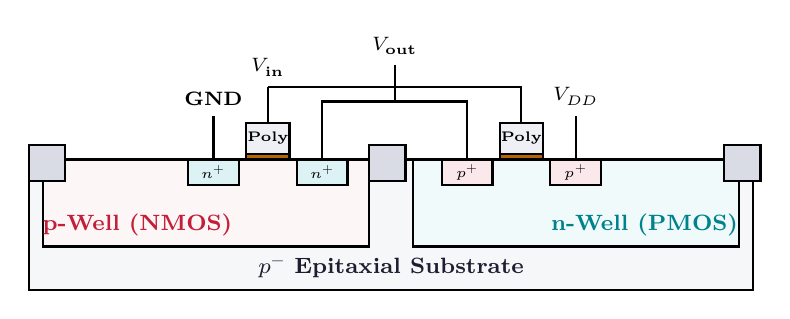
\begin{tikzpicture}[scale=0.92]
  % Substrate
  \draw[thick, fill=mygray] (-5.0, -1.8) rectangle (5.0, 0);
  \node[font=\footnotesize\bfseries\color{mydark}] at (0, -1.5) {$p^-$ Epitaxial Substrate};

  % P-Well (Left)
  \draw[thick, fill=hdrred!40] (-4.8, -1.2) rectangle (-0.3, 0);
  \node[font=\footnotesize\bfseries\color{myred}] at (-3.5, -0.9) {p-Well (NMOS)};

  % N-Well (Right)
  \draw[thick, fill=hdrteal!40] (0.3, -1.2) rectangle (4.8, 0);
  \node[font=\footnotesize\bfseries\color{myteal}] at (3.5, -0.9) {n-Well (PMOS)};

  % STI Isolation Oxide
  \foreach \x in {-5.0, -0.3, 4.6} {
    \draw[thick, fill=mgframe!50] (\x, -0.3) rectangle (\x+0.5, 0.2);
  }

  % NMOS Sources/Drains n+
  \draw[thick, fill=hdrteal] (-2.8, -0.35) rectangle (-2.1, 0) node[midway, font=\tiny\bfseries] {$n^+$};
  \draw[thick, fill=hdrteal] (-1.3, -0.35) rectangle (-0.6, 0) node[midway, font=\tiny\bfseries] {$n^+$};

  % NMOS Gate
  \draw[thick, fill=myamber] (-2.0, 0) rectangle (-1.4, 0.08); % Gate oxide
  \draw[thick, fill=hdrgray] (-2.0, 0.08) rectangle (-1.4, 0.5) node[midway, font=\tiny\bfseries] {Poly};

  % PMOS Sources/Drains p+
  \draw[thick, fill=hdrred] (0.7, -0.35) rectangle (1.4, 0) node[midway, font=\tiny\bfseries] {$p^+$};
  \draw[thick, fill=hdrred] (2.2, -0.35) rectangle (2.9, 0) node[midway, font=\tiny\bfseries] {$p^+$};

  % PMOS Gate
  \draw[thick, fill=myamber] (1.5, 0) rectangle (2.1, 0.08); % Gate oxide
  \draw[thick, fill=hdrgray] (1.5, 0.08) rectangle (2.1, 0.5) node[midway, font=\tiny\bfseries] {Poly};

  % Contact terminals
  \draw[thick] (-1.7, 0.5) -- (-1.7, 1.0) node[above, font=\scriptsize\bfseries] {$V_{\text{in}}$};
  \draw[thick] (1.8, 0.5) -- (1.8, 1.0) -- (-1.7, 1.0);
  \draw[thick] (-0.95, 0) -- (-0.95, 0.8) -- (1.05, 0.8) -- (1.05, 0);
  \draw[thick] (0.05, 0.8) -- (0.05, 1.3) node[above, font=\scriptsize\bfseries] {$V_{\text{out}}$};
  \draw[thick] (-2.45, 0) -- (-2.45, 0.6) node[above, font=\scriptsize\bfseries] {GND};
  \draw[thick] (2.55, 0) -- (2.55, 0.6) node[above, font=\scriptsize\bfseries] {$V_{DD}$};
\end{tikzpicture}
\end{tcolorbox}

\newpage
% ===============================================================================
% MANDATORY QUICK REVISION PAGE
% ===============================================================================
\begin{center}
  {\large\bfseries\color{myred} Quick Revision --- Module 4}\\[3pt]
  {\small\color{mydark} Opto-Electronics \& Integrated Circuit Fabrication $|$ EC301}
\end{center}
\noindent{\color{myred}\rule{\linewidth}{1.2pt}}
\vspace{4pt}

\begin{tcolorbox}[formulabox, title={\textbf{Key Formulas and Metrics at a Glance}}]
\renewcommand{\arraystretch}{1.35}
\begin{tabularx}{\linewidth}{B{5.0cm} X}
Optical Absorption Cut-off & $\lambda_c = \frac{hc}{E_g} = \frac{1.24}{E_g\,(\text{eV})}\,\mu\text{m}$ \\[4pt]
Beer-Lambert Law & $I(x) = I_0 \exp(-\alpha x)$ \\[4pt]
Solar Cell Open-Circuit Voltage & $V_{oc} = \eta V_T \ln\left(\frac{I_L}{I_0} + 1\right)$ \\[4pt]
Solar Cell Fill Factor ($FF$) & $FF = \frac{V_m I_m}{V_{oc} I_{sc}}$ \\[4pt]
Solar Cell Power Efficiency ($\eta$) & $\eta = \frac{V_m I_m}{P_{\text{in}}} = \frac{V_{oc} I_{sc} FF}{P_{\text{in}}}$ \\[4pt]
Photoconductive Gain ($G$) & $G = \frac{\tau}{t_{\text{transit}}} = \frac{\tau \mu V}{L^2}$ \\[4pt]
Photodiode Responsivity ($R$) & $R = \frac{I_{\text{photo}}}{P_{\text{opt}}} = \frac{\eta_{ext} q \lambda}{hc}$ \\[4pt]
Phototransistor Collector Current & $I_C = (\beta + 1) I_{\text{photo}}$ \\[4pt]
Laser Population Inversion & $E_{Fn} - E_{Fp} > h\nu > E_g$ \\[4pt]
APD Multiplication Factor ($M$) & $M = \frac{1}{1 - (V_R / V_{BR})^n}$ \\[4pt]
\end{tabularx}
\end{tcolorbox}

\begin{tcolorbox}[defbox, title={\textbf{One-Line Definitions}}]
\begin{itemize}[leftmargin=*, itemsep=2pt, topsep=0pt]
  \item \textbf{Photovoltaic Effect:} Direct generation of electric potential across a p-n junction caused by absorption of incident photons.
  \item \textbf{Fill Factor ($FF$):} Figure of merit measuring the squareness of a solar cell's fourth-quadrant I-V characteristic.
  \item \textbf{PIN Photodiode:} High-speed, high-efficiency photodetector incorporating a wide intrinsic layer between $p^+$ and $n^+$ regions.
  \item \textbf{Avalanche Photodiode (APD):} Highly sensitive photodetector employing internal carrier multiplication via impact ionization.
  \item \textbf{Population Inversion:} Non-equilibrium condition where the number of electrons in higher energy states exceeds that in lower states.
  \item \textbf{Photolithography:} Microfabrication process transferring photographic geometrical circuit patterns onto a photosensitive polymer resist.
  \item \textbf{Dry Reactive Ion Etching (RIE):} High-resolution anisotropic material removal combining chemical reactivity with directional ion bombardment.
  \item \textbf{Chemical Vapor Deposition (CVD):} Deposition of high-purity solid dielectric or polysilicon thin films from vapor-phase chemical precursors.
\end{itemize}
\end{tcolorbox}

\begin{tcolorbox}[exambox, title={\textbf{Frequently Asked / Viva Questions}}]
\begin{enumerate}[topsep=0pt, label=\textbf{Q\arabic*.}, itemsep=5pt]
  \item \Q{Why does a PIN photodiode possess significantly higher speed and bandwidth than a standard p-n photodiode?}
    In a standard p-n diode, many carriers are generated in neutral regions and must slowly diffuse to the junction ($t_{\text{diff}} \sim \mu\text{s}$). In a PIN diode, the wide intrinsic layer ($W_i$) ensures nearly all photons are absorbed directly within the depletion field, where carriers drift at saturation velocity ($t_{\text{drift}} \sim \text{ps}$). Furthermore, the wide layer significantly reduces junction capacitance ($C_j = \epsilon A / W_i$), decreasing the $RC$ time constant.
  \item \Q{What is the difference between spontaneous emission and stimulated emission?}
    Spontaneous emission occurs randomly without external influence, yielding photons of arbitrary direction and incoherent phase (LED operation). Stimulated emission is triggered by an incoming photon, causing an excited electron to drop and emit a twin photon with identical wavelength, phase, direction, and polarization (Laser operation).
  \item \Q{State the necessary conditions for semiconductor laser operation.}
    \begin{itemize}[leftmargin=*, itemsep=1pt, topsep=2pt]
      \item Population inversion across the bandgap ($E_{Fn} - E_{Fp} > h\nu > E_g$).
      \item Optical cavity feedback (Fabry-Perot resonator) to sustain stimulated emission.
      \item Injection current density exceeding the threshold current density ($J > J_{th}$) where optical gain exceeds cavity losses.
    \end{itemize}
  \item \Q{What is the physical meaning of the Solar Cell Fill Factor ($FF$)?}
    It is the ratio of maximum achievable electric power ($V_m I_m$) to the ideal product ($V_{oc} I_{sc}$). A higher fill factor (approaching $0.85$) represents lower internal series resistance ($R_s \to 0$) and higher shunt resistance ($R_{sh} \to \infty$).
  \item \Q{Why is dry oxidation preferred over wet oxidation for gate oxide growth?}
    Dry oxidation ($\text{Si} + \text{O}_2 \to \text{SiO}_2$) grows very slowly, producing a dense, highly uniform, defect-free oxide film with extremely low interface trap density, which is critical for thin gate dielectrics. Wet oxidation ($\text{Si} + 2\text{H}_2\text{O} \to \text{SiO}_2 + 2\text{H}_2$) is much faster but yields a less dense oxide used for thick masking and field isolation.
  \item \Q{Compare Ion Implantation with Thermal Diffusion for junction doping.}
    Ion implantation allows independent, ultra-precise control over dopant dose and penetration depth, operates at low temperatures, and avoids lateral diffusion under mask edges. Thermal diffusion requires high temperatures ($>1000^\circ\text{C}$), suffers from lateral diffusion, but causes no crystal lattice damage.
  \item \Q{What is the difference between isotropic and anisotropic etching?}
    Isotropic etching (wet chemical) etches equally in all directions, causing significant mask undercut. Anisotropic etching (dry plasma / RIE) etches preferentially in the vertical direction, producing vertical sidewalls essential for sub-micron VLSI layouts.
  \item \Q{Why is the twin-tub CMOS process preferred over single-well CMOS?}
    In single-well CMOS, only one transistor type's well doping can be optimized; the other must use the substrate doping. In the twin-tub process, both n-well and p-well doping profiles and depths can be optimized independently, allowing precise matching of NMOS and PMOS threshold voltages and minimizing latch-up.
  \item \Q{What is photoconductive gain and how can it exceed unity?}
    $G = \tau / t_{\text{transit}}$. When the minority carrier lifetime $\tau$ exceeds the electron transit time $t_{\text{transit}}$, an electron sweeps out of the positive contact while an electron is simultaneously injected from the negative contact to maintain neutrality. The electron circulates through the external circuit multiple times before recombination occurs.
  \item \Q{What is the role of self-alignment in polysilicon gate MOS fabrication?}
    The polysilicon gate electrode acts as an implantation mask for the source and drain implants. This ensures that the edges of the source and drain line up with the edges of the gate, eliminating parasitic gate-to-source and gate-to-drain overlap capacitances.
\end{enumerate}
\end{tcolorbox}

\begin{tcolorbox}[tikzbox, title={Comparison of LED vs. Semiconductor Laser Diode}]
\centering
\renewcommand{\arraystretch}{1.45}
\begin{tabularx}{\linewidth}{|B{3.2cm}|Y|Y|}
\hline
\multicolumn{1}{|c|}{\textbf{Parameter}} & \multicolumn{1}{c|}{\textbf{Light Emitting Diode (LED)}} & \multicolumn{1}{c|}{\textbf{Semiconductor Laser Diode}} \\
\hline
Emission Mechanism & Spontaneous radiative recombination & Stimulated emission with optical cavity feedback \\
\hline
Coherence & Incoherent (random phases) & Highly coherent (identical phase and frequency) \\
\hline
Spectral Width ($\Delta \lambda$) & Wide ($\Delta \lambda \sim 25\text{--}50\,\text{nm}$) & Extremely narrow ($\Delta \lambda \sim 0.1\text{--}2\,\text{nm}$, monochromatic) \\
\hline
Beam Divergence & Wide, non-directional ($\sim 60\text{--}120^\circ$) & Narrow, highly directional ($\sim 5\text{--}15^\circ$) \\
\hline
Threshold Current & No threshold current (emits light at any forward current) & Requires injection current exceeding threshold $I_{th}$ \\
\hline
Modulation Bandwidth & Moderate (tens to hundreds of $\text{MHz}$) & Ultra-high (tens of $\text{GHz}$) \\
\hline
Coupling Efficiency & Low coupling efficiency into optical fibers & High coupling efficiency ($> 80\%$) into single-mode fibers \\
\hline
Applications & Indicators, lighting, short-range plastic fibers & High-speed long-haul optical fiber communications, LiDAR \\
\hline
\end{tabularx}
\end{tcolorbox}

\end{document}
